\section{Performance Optimizations}\label{sec:optimizations}

Before comparing \iblock{}'s performance to other blockchain simulators,
profiling and optimizing the software were essential to identify and address
potential bottlenecks.

The Valgrind tool suite's \texttt{callgrind} profiler was employed to analyze
performance bottlenecks, with the results visualized through the KCacheGrind
tool \cites{callgrind, valgrind}. As shown in \figref{fig:callgrind}, the call
graph reveals key areas consuming execution time. Running a 5-hour simulation
with 30 nodes on an Intel Core i7-8705G CPU at \(4.1\) GHz (in debug mode under
the profiler) took 26 minutes and 17 seconds, providing a baseline for
optimization efforts.

\begin{figure}[tbhp]
	\centering
	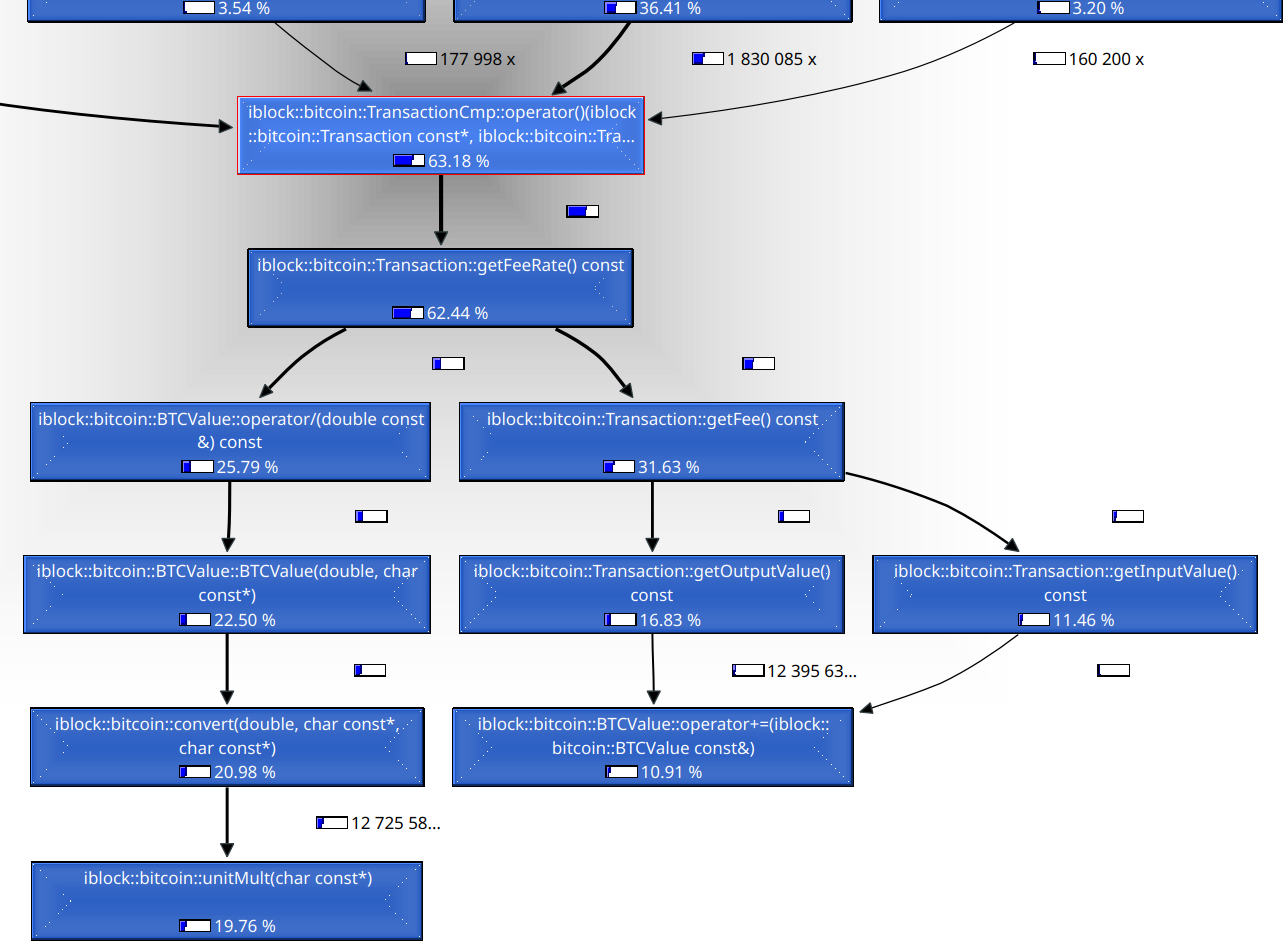
\includegraphics[width=\textwidth]{initial-callgraph}
	\caption{Part of the call graph of \iblock{}, before optimizations are
	applied.}\label{fig:callgrind}
\end{figure}

These optimizations described in this section collectively improved \iblock{}'s
efficiency, laying a strong foundation for performance evaluations against
other blockchain simulators.

\subsection{Reducing Calls to the Unit Conversion
Function}\label{subsec:reducing-convert-calls}

The profiling results in \figref{fig:callgrind} showed that a significant
portion of the simulation time (over 62\%) was consumed by the
\code{Transaction::getFeeRate()} function. This function is heavily used by the
\code{MempoolManager}'s comparator to maintain transaction ordering in the
mempool based on fee rates, allowing the miner to prioritize the most
profitable transactions.

Upon further analysis, half of this function's runtime was spent in
\code{getFee()} and the other half in calculating divisions between two
\code{BTCValue} instances. The \code{BTCValue} class provides flexible unit
support for Bitcoin values, enabling different units to be specified during
simulation configuration. However, every binary operation between two
\code{BTCValue} instances calls the \code{convert()} function twice --- once
for each instance --- to convert them to satoshis before performing the
operation.

To improve performance, the code was adjusted to skip the \code{convert()}
function call when both values are already in the same unit, thereby avoiding
unnecessary conversions. This optimization led to a considerable reduction in
runtime, bringing the simulation time for the same scenario down to 15 minutes
and 35 seconds.

\subsection{Caching Values in the Transaction
Class}\label{subsec:caching-values}

Further optimization targeted the \code{Transaction} class, which frequently
retrieves the fee, fee rate (fee per byte), and total input and output values
of transactions. Previously, these values were recalculated every time the
associated getter functions were called, with fees computed by subtracting
total output from total input values, which themselves were summed by iterating
over all transaction inputs and outputs.

In order to streamline these computations, four caching variables were added to
the \code{Transaction} class to store these frequently accessed values. This
enhancement decreased the simulation time to 11 minutes and 55 seconds, marking
a notable improvement by reducing redundant calculations.

\subsection{Optimizing the TransactionGenerator Application}\label{subsec:optimizing-txgen}

The optimized call graph of the simulator, shown in
\figref{fig:callgrind-optimized}, indicates that a significant portion of time
--- nearly 50\% --- is now spent in the \code{createTransaction()} function of
the \code{TransactionGenerator} class. This behavior is expected, as
transaction generation and propagation are core tasks of the simulator, with
transactions created frequently compared to occasional block production.

\begin{figure}[tbhp]
	\centering
	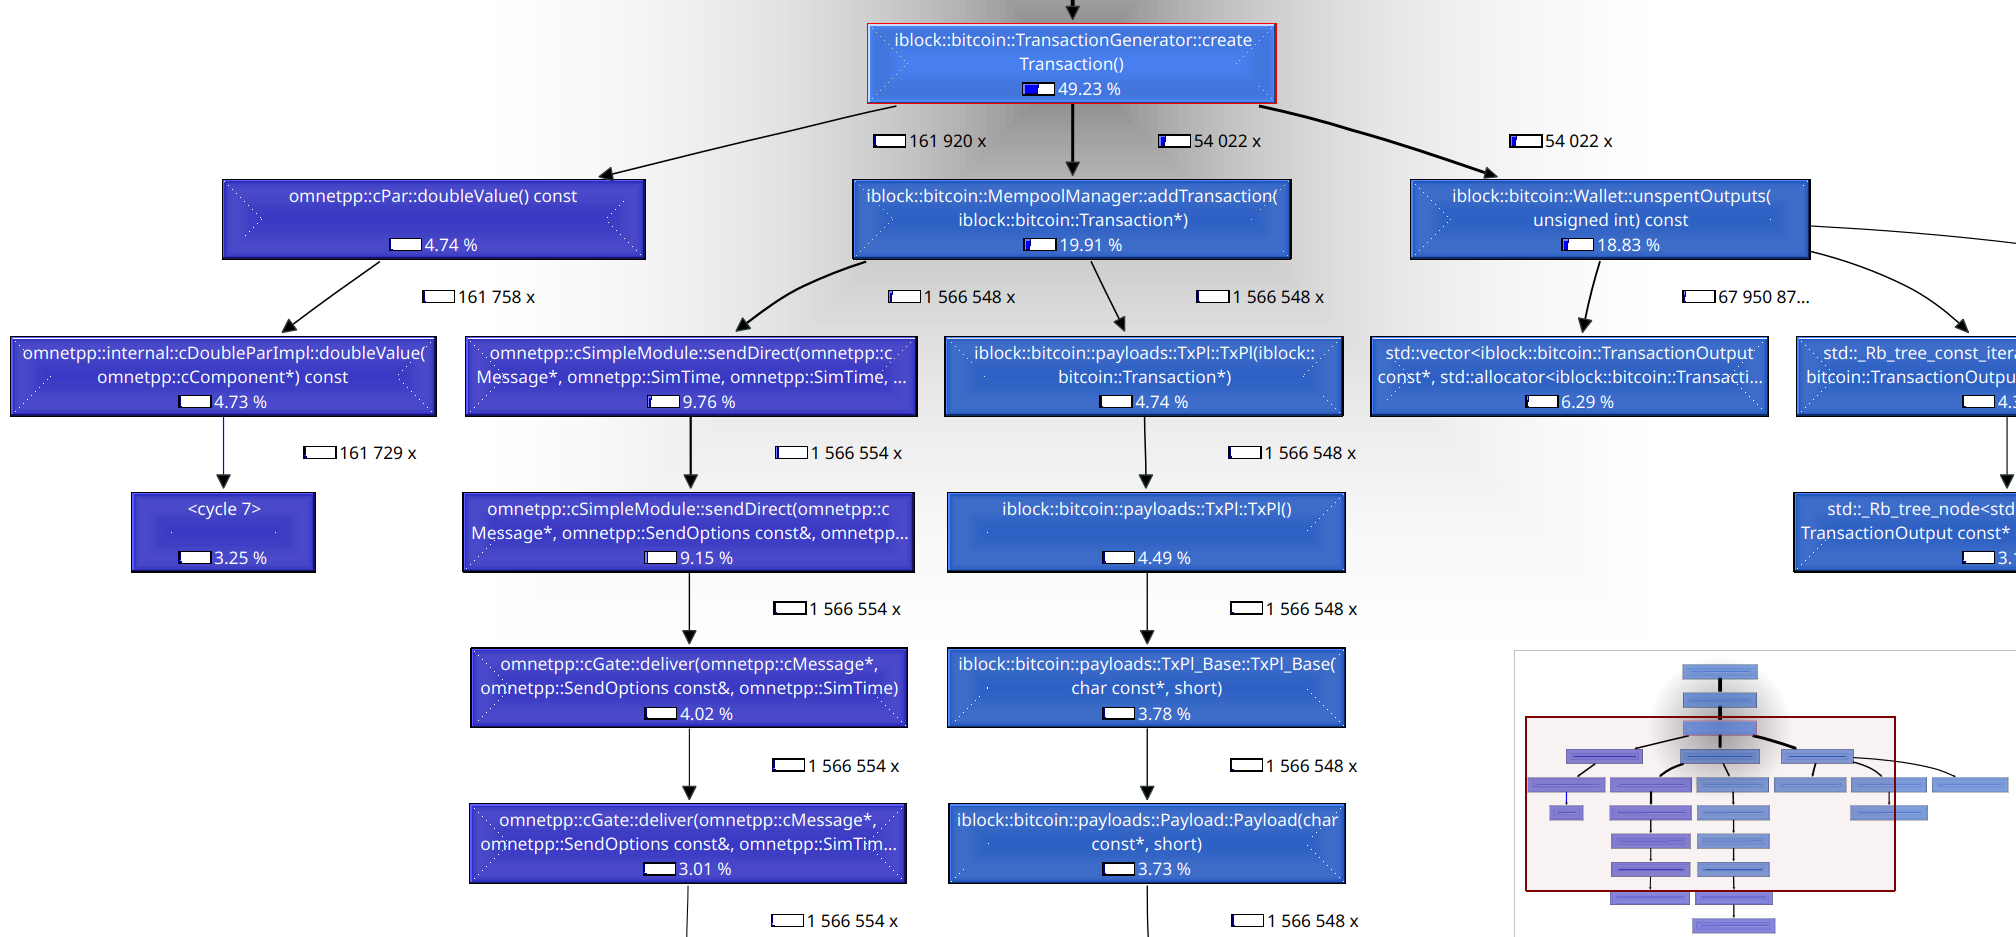
\includegraphics[width=\textwidth]{optimized-callgraph}
	\caption{Part of the call graph of \iblock{}, after optimizations are
	applied.}\label{fig:callgrind-optimized}
\end{figure}

Despite these optimizations, additional improvements are possible. Currently,
every time the \code{createTransaction()} function is called, it checks the
wallet's balance to ensure sufficient funds for the transaction by iterating
over all \textit{Unspent Transaction Outputs} (UTXOs) and summing their values.

To reduce these balance checks, we introduced a mechanism where the
transaction generator application pauses its timer when the wallet balance is
insufficient. The \code{Wallet} can then notify the \code{TransactionGenerator}
to resume through a callback when the balance is updated. This functionality is
implemented in the \code{notifyOnBalanceIncrease()} function of the
\code{Wallet} class, reducing unnecessary balance checks and allowing for more
efficient operation.

Although caching the balance was considered, it was ultimately deemed
impractical due to the variable nature of what constitutes ``spendable''
balance --- UTXOs may be considered spendable after a variable number of
confirmations, tipically determined in the real world by the user of the wallet
program and its confidence that transactions with a low number of confirmations
will not be thrown out of the blockchain. To support custom input selection
policies for transactions, the \code{Wallet} class refrains from directly
storing the balance.

